\chapter{Języki i~metody programowania}
\PartialToc
%\startcontents[chapters]
%\printcontents[chapters]{}{1}{\section*{\contentsname}}
\section{IT1A\_W03,IT1A\_U03,IT1A\_U07}
\textbf{W~jaki sposób można obliczyć długość tekstu przekazanego jako argument w~poniższej funkcji?}
\begin{lstlisting}[language=c]
void foo(const char* txt) {
. . .
}
\end{lstlisting}
\subsection{Odpowiedź}

\begin{itemize}
\item Używając funkcji strlen z biblioteki string.h
\begin{lstlisting}[language=c]
/* Declaration */
size_t strlen(const char *str)

/* Example */
strlen(txt)
\end{lstlisting}

\item Zliczając ile znaków występuje w tekście od znaku na który wskazuje wskaźnik do znaku końca łańcucha znaków ('\textbackslash0')
\begin{lstlisting}[language=c]
int length = 0;
char c = *txt;
while(c != '\0') {
   length++;
   c = *(++txt);
}
\end{lstlisting}
\end{itemize}
  
\subsection{Wprowadzenie teoretyczne}
\textbf{Łańcuch znaków}\\
Łańuch znaków w języku C to tablica znaków której ostatni element ma wartość \textbackslash0 - null\\
Poniższe deklaracje łańcucha znaków są równoważne:
\begin{lstlisting}[language=c]
char greeting[]  = "Hello";
char greeting[6] = "Hello";
char *greeting   = "Hello";
char greeting[]  = { 'H', 'e', 'l', 'l' 'o', '\0'};
char greeting[6] = { 'H', 'e', 'l', 'l' 'o', '\0'};
\end{lstlisting}

\begin{center}
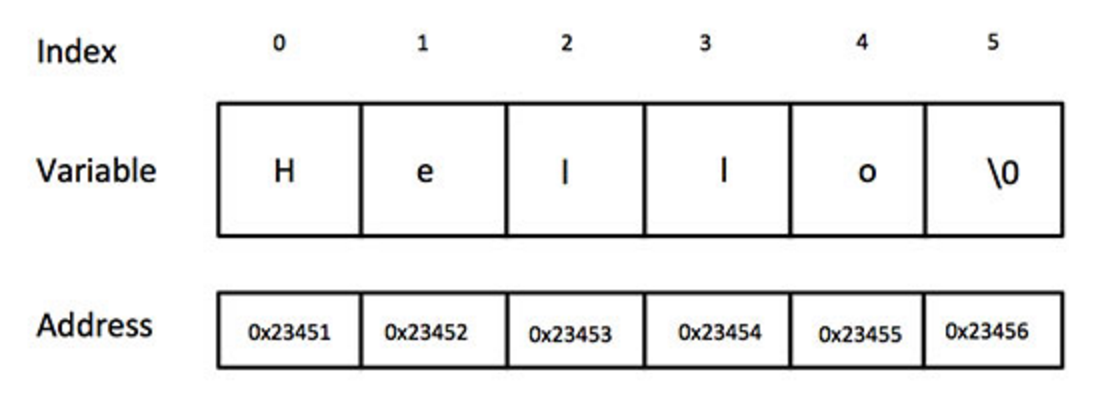
\includegraphics[width=13cm]{string_in_c}
\captionof{figure}{Łańcuchy znaków w C}
\end{center}

Istnieje biblioteka string.h która zawiera funkcja ułatwiające manipulowanie łańcuchami znaków.
\begin{lstlisting}[language=c]
strcpy(s1, s2); 
/*Copies string s2 into string s1*/

strcat(s1, s2);
/*Concatenates string s2 onto the end of string s1*/

strlen(s1);
/*Returns the length of string s1*/

strcmp(s1, s2);
/*Returns 0 if s1 and s2 are the same; less than 0 if s1<s2; greater than 0 if s1>s2*/
\end{lstlisting}

% 2 ---------------------------------------------------------------------------------------------------------------

\section{IT1A\_W03,IT1A\_U03,IT1A\_U07}dassdas

% 3 ---------------------------------------------------------------------------------------------------------------

\section{IT1A\_W03,IT1A\_U03,IT1A\_U07} 
\textbf{W jaki sposób obliczyć długość tablicy w funkcji foo()?}
\begin{lstlisting}[language=c]
void foo(double t[]){
   // dlugosc tablicy t?
}
\end{lstlisting}

\subsection{Odpowiedź}
\begin{itemize}
\item W tym wypadku nie jest możliwe obliczenie długości tablicy.\\
\end{itemize}

\subsection{Wprowadzenie teoretyczne}
Nie jest możliwe obliczenie długości tablicy posiadając jedynie wskaźnik do niej.\\
Kompilator języka C potrafi obliczyć długość tablicy jeżeli została ona zadeklarowana w tej samej metodzie w której chcemy sprawdzić długość tablicy:
\begin{lstlisting}[language=c]
int array[] = { 1, 2, 3, 4 };
int n = sizeof(array) / sizeof(array[0]);
printf("Array has %d elements\n", n); /* it should returns 4 */

foo(array);
/*...*/
void foo(int t[]){
   int n = sizeof(t) / sizeof(t[0]);
   printf("Array has %d elements\n", n); /* it shouldn't returns 4 */
}
\end{lstlisting}

% 4 ---------------------------------------------------------------------------------------------------------------

\section{Pytanie 4}dassdas

% 5 ---------------------------------------------------------------------------------------------------------------

\section{IT1A\_W03,IT1A\_U03,IT1A\_U07}
\textbf{Zakładając, ze wielkość typu char to jeden bajt, short to dwa bajty, a double to osiem bajtów, jaka jest wartość wyrażenia sizeof(x), gdzie x jest zmienną poniższego typu strukturalnego, dla standardowych ustawień kompilatora 32-bitowego?}
\begin{lstlisting}[language=c]
struct {
   char c;
   short i;
   double d;
} x;
\end{lstlisting}

\subsection{Wstęp teoretyczny}
W języku C każdy typ, oprócz char jest dopasowywany odpowiednio w przestrzeni adresowej.
\begin{itemize}
\item char może mieć początek na każdym bajcie w przestrzeni adresowej
\item short musi mieć początek na adresie parzystym
\item int lub float musi mieć początek na adresie podzielnym przez 4
\item long musi mieć początek na adresie podzielnym przez 8
\end{itemize}
\textbf{Przykład ułożenia zmiennych w pamięci: }
\begin{lstlisting}[language=c]
char *p;
char c;
int x;
\end{lstlisting}
Przestrzeń dla p zajmuje 4 bajty, zaraz po nim mamy chara 1 bajtowego. Ale rozmieszczenie 4-bajtowego x wymaga dodania luki:

\begin{lstlisting}[language=c]
char *p;      /* 4 or 8 bytes */
char c;       /* 1 byte */
char pad[3];  /* 3 bytes */
int x;        /* 4 bytes */
\end{lstlisting}
pad[3] reprezentuje fakt, że int musi zacząć się na adresie wielokrotności 4. \\\\
\textbf{Pierwszy przykład dla struktur (maszyna 64-bitowa)}
\begin{lstlisting}[language=c]
struct foo1 {
   char *p;     /* 8 bytes */
   char c;      /* 1 byte
   char pad[7]; /* 7 bytes */
   long x;      /* 8 bytes */
};
\end{lstlisting}
\textbf{Drugi przykład dla struktur}
\begin{lstlisting}[language=c]
struct MixedData  /* After compilation in 32-bit x86 machine */
{
    char Data1; /* 1 byte */
    char Padding1[1]; /* 1 byte for the following 'short' to be aligned on a 2 byte boundary
assuming that the address where structure begins is an even number */
    short Data2; /* 2 bytes */
    int Data3;  /* 4 bytes - largest structure member */
    char Data4; /* 1 byte */
    char Padding2[3]; /* 3 bytes to make total size of the structure 12 bytes */
};
\end{lstlisting}
Wydawaćby się mogło, że sizeof(MixedData) = 9. Jednak nie - rozmiar struktury wynosi 12 bajtów! Do ostatniego elementu struktury dodany jest padding, dzięki któremu rozmiar struktury będzie wielokrotnością największego elementu struktury (tutaj int - 4 bajty). \\\\
\textbf{Odpowiedź na pytanie} \\
sizeof(x) = 1 + padding(1) + 2 + padding(4) + 8 = 16 

% 6 ---------------------------------------------------------------------------------------------------------------

\section{Pytanie 6}dassdas

% 7 ---------------------------------------------------------------------------------------------------------------

\section{IT1A\_W03,IT1A\_U03,IT1A\_U07} 
\textbf{Przeanalizuj poniższą deklarację w języku C}
\begin{lstlisting}[language=c]
int (*x)(int, int);
\end{lstlisting}

\subsection{Odpowiedź}
\begin{itemize}
\item Deklaracja wskaźnika na funkcję przyjmującą jako parametr dwa integery\\
\end{itemize}

\subsection{Wprowadzenie teoretyczne}
\textbf{Wskaźniki na funkcje}\\
Każda funkcja tak jak i zmienna ma swoje miejsce w pamięci do którego można przypisać wskaźnik.\\
Wskaźnik na funkcje różni się od wskaźników na zmienne deklaracją:
\begin{lstlisting}[language=c]
typ_zwracanej_wartosci (*nazwa_wskaznika)(typ1 argument1, typ2 argument2, ...);
\end{lstlisting}
Przypisując nazwę funkcji bez nawiasów do wskaźnika automatycznie informujemy kompilator, że chodzi nam o adres funkcji.\\
Wskaźnika używamy tak, jak normalnej funkcji, na którą on wskazuje.\\
Przykład:
\begin{lstlisting}[language=c]
#include <stdio.h>

int suma (int lhs, int rhs){
   return lhs+rhs;
}
 
int main (){
   int (*wsk_suma)(int a, int b);
   wsk_suma = suma;
   printf("4+5=%d\n", wsk_suma(4,5));
   return 0;
}
\end{lstlisting}
